\chapter{简要~\LaTeX~使用说明}\label{cha:latex-brief-intro}

\section{控制单位}

LaTeX里可使用的单位包括:
\begin{itemize}
    \item 毫米\ \verb|1mm|
    \item 厘米\ \verb|1cm|
    \item 英寸\ \verb|1in|
    \item 像素\ \verb|1pt|
    \item 基础文本尺寸的宽度\ \verb|1em|
    \item 基础文本尺寸的高度\ \verb|1ex|
    \item 字符宽度或行宽度的百分比值\ \verb|0.2\textwidth|
    \item 字符高度或行高度的百分比值\ \verb|0.2\textheight|
\end{itemize}

\section{特殊符号}

~\LaTeX~中有些符号无法正常显示,比如:\# \quad \% \quad \& \quad \{ \quad \} \quad \~{} \quad \_{} \quad \textbackslash \quad \backslash \quad \^{} \quad \$ 等控制符号,错误的在代码中使用会产生Error报错,并且很难发现错误原因。同时输入“\backslash 命令”时需注意,若命令结束后紧跟正文内容,需要在结尾加入空格,即\verb|a \quad b|。

发现Error报错后,请对刚才添加的内容进行错误排查,重点观察报错位置附近的特殊符号、插入图片的路径、代码 \} 大括号是否完整。若无法判断错误位置,可以将添加部分临时删除,一点一点的加入并编译,直至出现Error报错,缩小错误代码的位置。

\subsection{空白符号}

\paragraph*{~\LaTeX~空白的原则:}

\begin{itemize}
    \item 空行分段,多个空行等同为1个
    \item 段落首行缩进是自动的,绝对不能使用空格代替
    \item 英文中多个空格处理为1个空格,中文中空格将被忽略
    \item 汉字与其他字符的间距会自动有XeLaTeX处理
    \item 禁止使用中文全角空格
\end{itemize}

\paragraph*{空格的输入方法:}

\begin{itemize}
    \item 当前字体的一个宽度,即1em\\
    \verb|a \quad b| \quad a \quad b
    \item 2em空格\\
    \verb|a \qquad b| \quad a \qquad b
    \item 1/6em空格\\
    \verb|a \, b| \qquad \qquad  a\,b \\
    \verb|a \thinspace b| a \thinspace b
    \item 0.5em空格\\
    \verb|a \enspace b| \quad a \enspace b
    \item 空格\\
    \verb|a \ b| \quad a \ b
    \item 硬空格(不能分割\\
    \verb|a~b| \quad a~b
    \item 指定宽度的空白 (1pc=12pt=4.218mm)\\
    \verb|a \kern 1pc b| \ \qquad a\kern 1pc b\\
    \verb|a \kern -1em b| \qquad a\kern -1em b\\
    \verb|a \hskip 1em b| \qquad a\hskip 1em b\\
    \verb|a \hspace{35pt}b| \quad a\hspace{35pt}b
    \item 占位宽度 xyz的占位宽度\\
    \verb|a \hphantom{xyz}b| \quad a\hphantom{xyz}b
    \item 弹性宽度,占满横向空间\\
    \verb|a \hfill b| \quad a\hfill b
\end{itemize}
 
\subsection{文本控制}

\begin{itemize}
    \item 分段(有段首缩进) \\
    \verb|para1|\\ \hspace*{\fill} \\\verb|para2|

    para1

    para2

    \item 文字之间直接换行(无缩进)\\
    \verb|para1\\line2|

    para1\\line2

    \item 添加空白行(会出现Warning) \\
    \verb|line1 \\ ~\\ line2| \\
    line1 \\ ~\\ line2

    \item 这个命令也可以加空行(无Warning),一般用在文字之间加空行 \\
    \verb|line1 \\ \hspace*{\fill} \\ line2| \\
    line1\\ \hspace*{\fill} \\line2

    \item 控制空行高度 \\
    \verb|line1 \\ \vspace{5ex} \\ line2| \\
    line1 \\ \vspace{5ex} \\ line2

    \item 换页(新页包含段首缩进) \\
    \verb|line1 \newpage para2| \\
    line1 \newpage para2
\end{itemize}

 \subsection{\LaTeX 控制符}
 \begin{itemize}
    \item \verb|\#| \qquad \#
    \item \verb|\$| \qquad \$
    \item \verb|\%| \qquad \%
    \item \verb|\{| \qquad \{
    \item \verb|\}| \qquad \}
    \item \verb|\&| \qquad \&
    \item \verb|\~{}| \quad \~{}
    \item \verb|\_{}| \quad \_{}
    \item \verb|\^{}| \quad \^{}
    \item \verb|\textbackslash| \qquad \textbackslash
 \end{itemize}

 \subsection{排版符号}
 \S \P \dag \ddag \copyright \pounds

 \subsection{\TeX 标志符号}
 \LaTeX \TeX{}  \LaTeXe{}

 \subsection{引号}

 \paragraph*{半角输入模式:}

 \begin{itemize}
    \item \verb|`| \ \quad 左单引号:`        %(键盘第二行第一个)  
    \item \verb|'|  \ \quad 右单引号:' 
    \item \verb|``| \quad 左双引号:`` 
    \item \verb|''| \quad 右双引号:'' 
 \end{itemize}

 \paragraph*{全角输入模式:}

\begin{itemize}
    \item  ‘  \ \quad 左单引号:‘ 
    \item  ’  \ \quad 右单引号:’ 
    \item  \verb|“| \ \quad 左双引号:“ 
    \item  \verb|”| \ \quad 右双引号:” 
\end{itemize}

 \subsection{连字符}

\begin{itemize}
    \item \verb|-| \ \ \ \quad -
    \item \verb|--| \ \ \quad --
    \item \verb|---| \quad ---
\end{itemize}

\section{各节一级标题 section}

\textbf{注意:命令不带*会显示编号,带*则不进行编号}

\subsection{各节二级标题 subsection}
你是内容

\subsection*{无编号二级标题 subsection*}
content

\subsubsection{各节三级标题 subsubsection}
他是内容

\paragraph{四级标题 paragraph}
内容内容

\subparagraph{五级标题 subparagraph}
内容内容

\section{字体样式}

\subsection{字体调节}

\begin{tabular}{ll}
	\verb|\songti|   & {\songti 宋体}   \\
	\verb|\heiti|    & {\heiti 黑体}    \\
	\verb|\fangsong| & {\fangsong 仿宋} \\
	\verb|\kaishu|   & {\kaishu 楷书}
\end{tabular}


\subsection{字号调节}
字号命令: \verb|\zihao| \index{zihao}

\begin{tabular}{ll}
\verb|\zihao{0}| &\zihao{0}  初号字 English \\
\verb|\zihao{-0}|&\zihao{-0} 小初号 English \\
\verb|\zihao{1} |&\zihao{1}  一号字 English \\
\verb|\zihao{-1}|&\zihao{-1} 小一号 English \\
\verb|\zihao{2} |&\zihao{2}  二号字 English \\
\verb|\zihao{-2}|&\zihao{-2} 小二号 English \\
\verb|\zihao{3} |&\zihao{3}  三号字 English \\
\verb|\zihao{-3}|&\zihao{-3} 小三号 English \\
\verb|\zihao{4} |&\zihao{4}  四号字 English \\
\verb|\zihao{-4}|&\zihao{-4} 小四号 English \\
\verb|\zihao{5} |&\zihao{5}  五号字 English \\
\verb|\zihao{-5}|&\zihao{-5} 小五号 English \\
\verb|\zihao{6} |&\zihao{6}  六号字 English \\
\verb|\zihao{-6}|&\zihao{-6} 小六号 English \\
\verb|\zihao{7} |&\zihao{7}  七号字 English \\
\verb|\zihao{8} |&\zihao{8}  八号字 English \\
\end{tabular}

\subsection{字体样式}

注意:部分字体不支持会出现Warning警告,请根据实际情况进行使用。

宋体\quad \textbf{粗体}\quad \textit{斜体}\quad \textbf{\textit{粗斜体}}。

{\heiti 黑体\quad \textbf{粗体}\quad \textit{斜体}\quad \textbf{\textit{粗斜体}}}。

{\fangsong 仿宋\quad \textbf{粗体}\quad \textit{斜体}\quad \textbf{\textit{粗斜体}}}。

{\kaishu 楷书\quad \textbf{粗体}\quad \textit{斜体}\quad \textbf{\textit{粗斜体}}}。

Serif\quad \textit{Italic}\quad \textbf{Bold}\quad \textbf{\textit{BoldItalic}}

{\sffamily Sans\quad \textit{Italic}\quad \textbf{Bold}\quad \textbf{\textit{BoldItalic}}}

{\ttfamily Mono\quad \textit{Italic}\quad \textbf{Bold}\quad \textbf{\textit{BoldItalic}}}


\section{常用命令}

\begin{description}
  \item[cite]  参考文献引用, 得到形如 [3-7] 的样式。
  \item[color,xcolor]  支持彩色。
  \item[enumerate]  方便自由选择 enumerate 环境的编号方式。\\
  \textbf{详细说明请见\ref{sec:list}节。} \\
  比如

  \verb|\begin{enumerate}[(a)]| 得到形如 (a), (b), (c) 的编号。


  \verb|\begin{enumerate}[i)]| 得到形如 i), ii), iii) 的编号。

  \verb|\begin{enumerate}[\hspace{1cm}(1)]| \verb|\hspace|命令用于调整距离。

\end{description}

另外要说明的是, itemize, enumerate, description 这三种 list 环境,已经调节了其间距和缩进,
以符合中文书写的习惯。


\section{引用}

\textbf{详细说明请见\ref{cha:ref}节。}

参考文献的引用, 用命令~\verb|\cite{ }|。大括号内要填入的字串, 是自命名的文献条目名。参考文献建议使用文献管理工具进行管理,将所需文献导出bib格式,放于ref目录下,并在main.tex中引入。论文最后的参考文献会根据bib文件与实际cite的项目自动生成。

比如, 通常我们会说:

 {\kaishu
关于此问题, 请参见文献 \cite{oclc2000about}. 作者某某还提到了某某概念\upcite{xiaoyu2001chubanye}.}


上文使用的源文件为:

 {\kaishu
关于此问题, 请参见文献~\verb|\cite{oclc2000about}|. 作者某某还提到了某某概念~\verb|\upcite{xiaoyu2001chubanye}|.
}

其中~\verb|\upcite| 是自定义命令, 使文献引用呈现为\CJKunderdot{上标形式}.

({\heiti 注意:} {\kaishu 这里文献的引用, 有时需要以上标形式出现, 有时需要作为正文文字出现, 为什么?})

另外, 要得到形如~\cite{r1,r3,r4,r5} 的参考文献连续引用, 需要用到 cite 宏包(模板已经加入),
在正文中使用~\verb|\cite{r1,r3,r4,r5}| 的引用形式即可.
或者, 连续引用的上标形式: 使用~\verb|\upcite{r1,r2,r3}|, 得到\upcite{r1,r2,r3}。

若使用VSCode,修改了参考文献后一定要重新编译bib后再使用xe编译,否则cite部分会出现?,找不到引用的参考文献,同时最后参考文献部分也不会显示该引用。

\section{公式}

\textbf{详细说明请见\ref{sec:equation}节。}

公式书写可使用在线编辑器选择合适的命令:\url{https://www.latexlive.com/}

行内公式可使用\verb|$x=x^2$|,即$x=x^2$。

行间公式可使用equation环境,此时一般不建议空一行,会让公式产生缩进不居中。
\begin{equation}
x = 1.
\end{equation}

\section{图形与表格}

\subsection{图形}

\textbf{详细说明请见\ref{sec:figure}节。}

支持对~eps, pdf, jpg 等等常见图形格式。

再次\colorbox{red!45}{澄清一个误会}: \LaTeX{} 支持的图形格式绝非 eps 这一种。 无需特意把图片转化为 eps。

写实验报告时,像素图可直接使用jpg、png等常见格式,矢量图建议转换为pdf并进行适当裁剪后再插入。攥写学术论文时请根据具体刊物的要求插入相应图片。

用形如~\verb|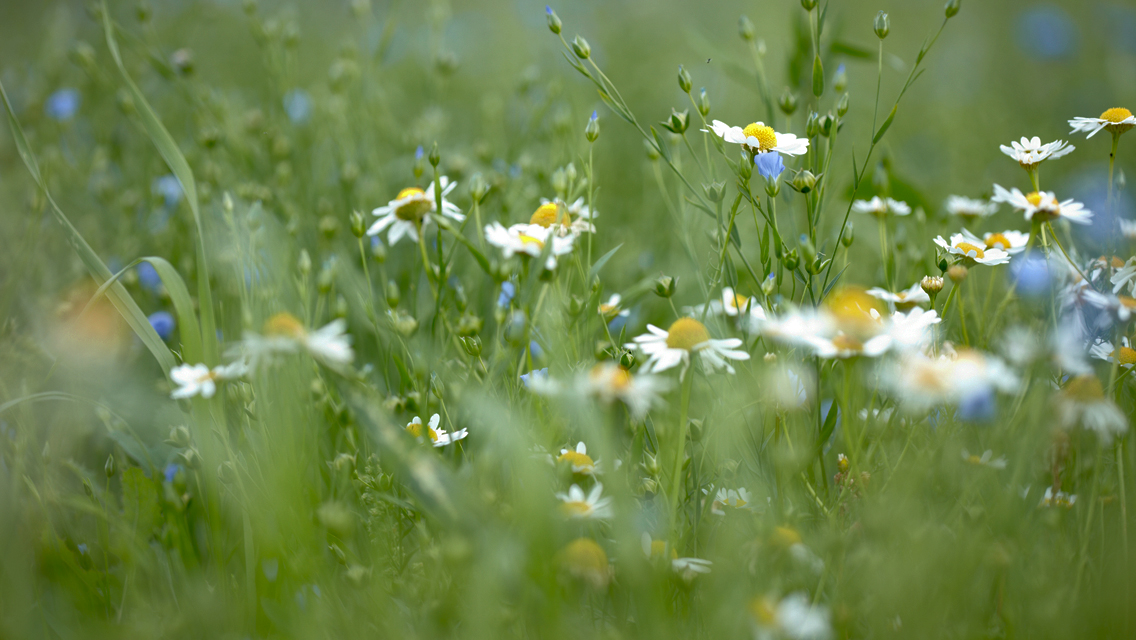
\includegraphics[width=12cm]{Daisy.jpg}| 的命令可以纳入图片。

如图~\ref{fig:1} 是一个纳入~jpg 图片的例子,\verb|[htb]|控制其位置,需要强制将图片放于代码所代表的位置时可以使用\verb|[H]|。

\begin{figure}[H]
\centering
  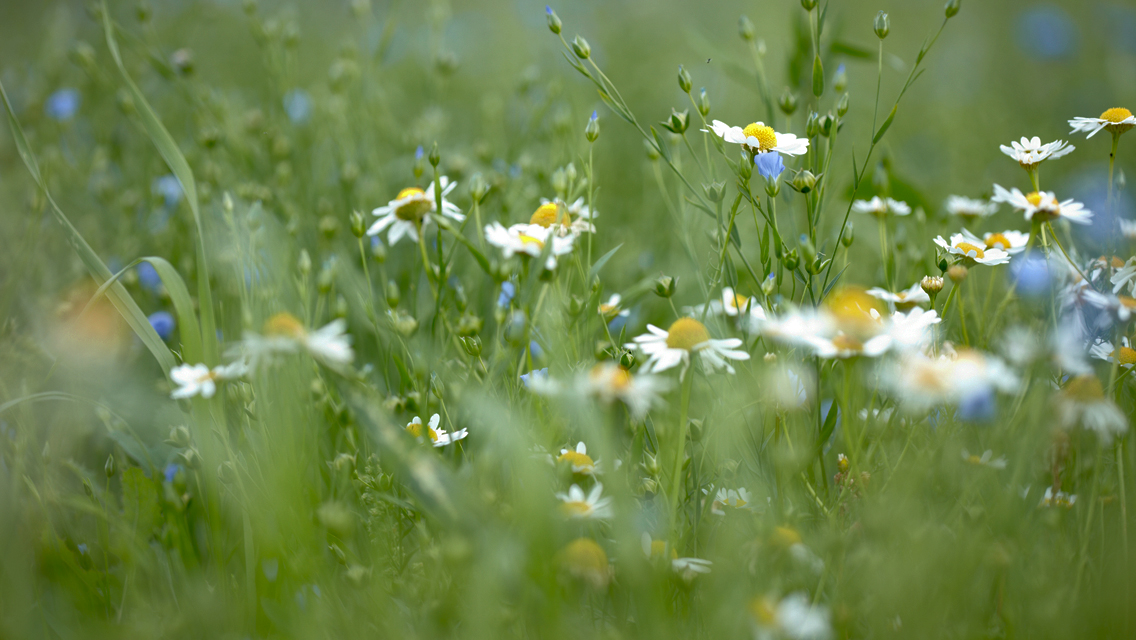
\includegraphics[width=\textwidth]{Daisy.jpg}
  \caption{一个彩色 jpg 图片的例子}
  \label{fig:1}
\end{figure}

\subsection{表格}

\textbf{详细说明请见\ref{sec:table}节。}

表格问题, 建议使用“三线表”, 如表 \ref{tab:1}。

\begin{table}[htb]
\centering
\caption{一般三线表}
\label{tab:1}
    \begin{tabular}{c c c c c c c c c c c}
    \hline
    123 & 4  & 5  & 123 & 4 & 5123 & 4 & 5 & 123 & 4 & 5\\
    \hline
    67 & 890 & 13 & 123 & 4 & 5123 & 4 & 5 & 123 & 4 & 5\\
    67 & 890 & 13 & 123 & 4 & 5123 & 4 & 5 & 123 & 4 & 5\\
    67 & 890 & 13 & 123 & 4 & 5123 & 4 & 5 & 123 & 4 & 5\\
    \hline
    \end{tabular}
\end{table}
